\documentclass[11pt]{article}

\usepackage[margin=1in]{geometry}
\usepackage{amsmath, amssymb}
\usepackage{graphicx}
\usepackage{booktabs}
\usepackage{hyperref}
\usepackage{xcolor}
\usepackage{caption}
\usepackage{subcaption}

\hfuzz=\maxdimen

\graphicspath{{../../figures/bpe_experiment/}}

\newcommand{\lcq}[1]{\textcolor{blue}{#1}}
\newcommand{\claude}[1]{{\color{red}\textsf{#1}}}
\newcommand{\old}[1]{{\color{gray}#1}}

\title{BPE Tokenization of HMM Sequences:\\
       Compression, Structure, and Time-Reversal}
\author{C.~L.}
\date{\today}

\begin{document}
\maketitle
\tableofcontents
\bigskip

%----------------------------------------------------------------------
\section{Introduction}
%----------------------------------------------------------------------

In previous experiments (see the Time-Reversal Symmetry report), transformers were trained directly on the raw emission alphabet of the Cylinder Graph HMM\@.  Each HMM observation token mapped one-to-one to a transformer input token, preserving the statistical structure of the process without distortion.  A natural follow-up question is: \emph{what happens when we interpose a learned tokenizer between the HMM and the transformer?}

Byte Pair Encoding (BPE) is the standard subword tokenization scheme used by essentially all large language models.  It greedily merges frequent character pairs into new tokens, producing a compressed representation in which each token carries more information than a single character.  When applied to HMM sequences, BPE faces a stationary ergodic source with known structure, making it possible to analyse what the tokenizer learns and how it reshapes the prediction problem.

This report documents the BPE tokenization pipeline for the Cylinder Graph HMM ($n{=}6$, depth${=}3$, $\alpha_{\mathrm{Dir}}{=}0.3$, $p{=}0.1$).  Section~\ref{sec:pipeline} describes the implementation.  Section~\ref{sec:merges} analyses the merge table and its relationship to the HMM's emission structure.  Section~\ref{sec:compression} characterises compression as a function of vocabulary size.  Section~\ref{sec:entropy} examines how BPE reshapes the entropy landscape.  Section~\ref{sec:reversal} describes the time-reversal experiment design.  Section~\ref{sec:discussion} discusses implications and open questions.

%----------------------------------------------------------------------
\section{Pipeline}\label{sec:pipeline}
%----------------------------------------------------------------------

The tokenize-then-train pipeline proceeds in four stages:

\begin{enumerate}
\item \textbf{Raw data generation.}  A single long sequence of $10^7$ HMM observation tokens is generated from the Cylinder Graph HMM and stored as a NumPy shard.  The raw alphabet has $|\mathcal{V}_{\mathrm{raw}}| = 48$ tokens (3 emission layers $\times$ 16 tokens per cluster).

\item \textbf{BPE training.}  Each HMM token $v \in \{0, \ldots, 47\}$ is mapped to a unique ASCII character via $v \mapsto \texttt{chr}(0\text{x}21 + v)$, converting the integer sequence to a character string.  The string is chunked into blocks of $10^4$ characters, and a BPE tokenizer is trained using the HuggingFace \texttt{tokenizers} library with target vocabulary size $|\mathcal{V}_{\mathrm{BPE}}| = 128$ (48 base characters + 80 learned merges).  No pre-tokenization is applied: each chunk is treated as a single ``word'', since HMM sequences have no whitespace or delimiter structure.

\item \textbf{Dataset preparation.}  The full raw sequence is encoded with the trained tokenizer, producing a compressed BPE token sequence.  This is chunked into non-overlapping windows of length $T+1 = 17$ (context length $T = 16$ plus one target token), shuffled, and split 99/1 into train/test sets.  A reversed dataset is produced by flipping each BPE token sequence along the time axis --- this is reversal at the \emph{BPE token level}, not the raw HMM token level.

\item \textbf{Training.}  A 4-layer transformer (embedding dimension 32, 2 attention heads, $d_{\mathrm{head}} = 16$, ReLU activation, $d_{\mathrm{MLP}} = 128$, tied embeddings) is trained on next-token prediction with cross-entropy loss.  Five seeds are run for each direction (forward and reversed BPE), with identical hyperparameters (lr $= 10^{-3}$, batch size 128, 10 epochs, cosine schedule).
\end{enumerate}

Round-trip integrity is verified: 100 random subsequences of length 200 are encoded and decoded, confirming exact reconstruction.  The implementation lives in \texttt{src/bpe\_tokenizer.py} (training), \texttt{src/prepare\_bpe\_data.py} (dataset creation), and \texttt{config/bpe\_config.yaml} / \texttt{config/bpe\_config\_reversed.yaml} (training configs).

%----------------------------------------------------------------------
\section{Merge Table Analysis}\label{sec:merges}
%----------------------------------------------------------------------

The trained BPE tokenizer produces 80 merges on top of the 48 base characters.  Two structural features stand out.

\subsection{Merge Length Distribution}

Of the 80 merges, 77 are bigrams (two raw HMM tokens) and only 3 are trigrams.  No merges of length $\geq 4$ are learned at this vocabulary size.  This reflects the relatively high entropy of the source: with 48 base tokens and Dirichlet-distributed emissions ($\alpha = 0.3$, producing sparse but not degenerate distributions), even the most frequent bigrams do not dominate enough to seed long merge chains.

\begin{figure}[ht]
\centering
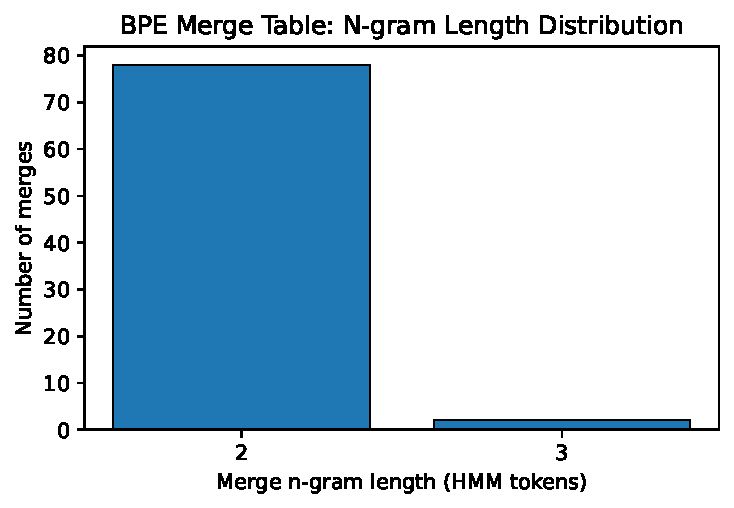
\includegraphics[width=0.55\textwidth]{merge_lengths.pdf}
\caption{Distribution of n-gram lengths in the 80 BPE merges.  Nearly all merges are bigrams; the source entropy is too high for longer merges to accumulate at $|\mathcal{V}| = 128$.}
\label{fig:merge-lengths}
\end{figure}

\subsection{Block-Diagonal Structure}

The Cylinder Graph HMM has three emission layers: tokens $0$--$15$ (layer 0), $16$--$31$ (layer 1), and $32$--$47$ (layer 2).  Each hidden state emits exclusively from its layer's token pool.  Figure~\ref{fig:merge-layers} shows that BPE merges are \emph{perfectly block-diagonal} in this layer structure: 24 merges within layer~0, 34 within layer~1, and 24 within layer~2, with zero cross-layer bigrams in the merge table.

This is expected: cross-layer bigrams correspond to transitions between different depth levels of the cylinder graph, and the transition probability $p = 0.1$ makes these relatively rare.  Within a layer, the hidden state cycles through positions $0, \ldots, n{-}1$ with high probability, producing strongly correlated consecutive emissions from the same token pool.  BPE captures exactly these within-layer correlations.

\begin{figure}[ht]
\centering
\begin{subfigure}[b]{0.48\textwidth}
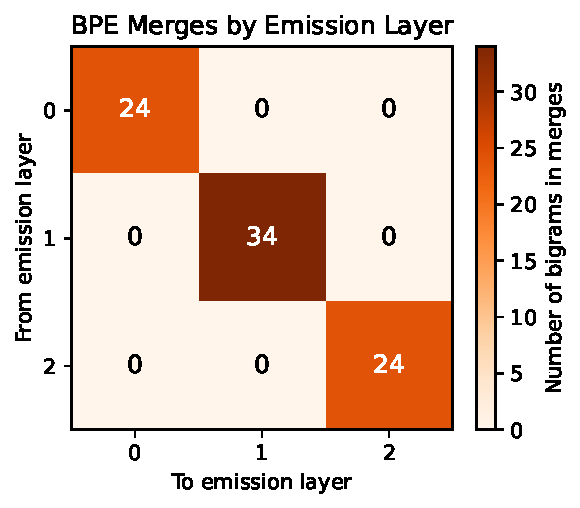
\includegraphics[width=\textwidth]{merge_layer_structure.pdf}
\caption{Merge bigram counts by emission layer.  The matrix is perfectly block-diagonal.}
\label{fig:merge-layers}
\end{subfigure}
\hfill
\begin{subfigure}[b]{0.48\textwidth}
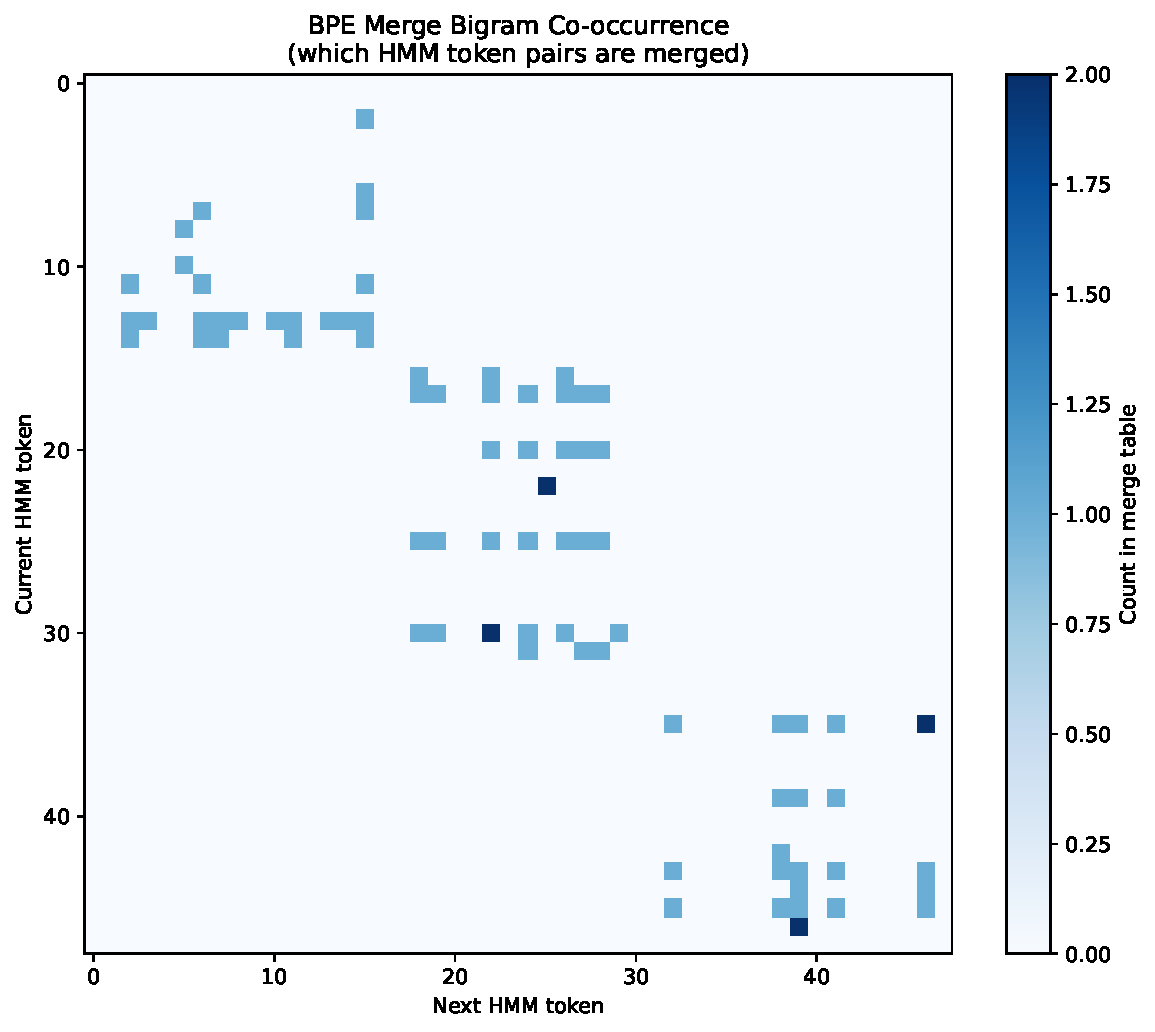
\includegraphics[width=\textwidth]{merge_cooccurrence.pdf}
\caption{Full $48 \times 48$ co-occurrence matrix of HMM token bigrams appearing in the merge table.}
\label{fig:merge-cooccur}
\end{subfigure}
\caption{BPE merge structure.  (a)~Aggregated by emission layer: all merges stay within layers, reflecting the HMM's block emission structure.  (b)~Token-level detail: the three diagonal blocks correspond to the three emission layers.}
\label{fig:merge-structure}
\end{figure}

The fact that BPE independently discovers the emission-layer partition --- without any supervision --- is a mild but clean demonstration that the tokenizer reflects genuine statistical structure of the source.  It also means that BPE tokens remain ``pure'' with respect to the emission layer: each merged token can be unambiguously assigned to a single layer.

%----------------------------------------------------------------------
\section{Compression}\label{sec:compression}
%----------------------------------------------------------------------

Figure~\ref{fig:compression} shows the compression ratio (raw tokens / BPE tokens) as a function of vocabulary size.  At the operating point $|\mathcal{V}| = 128$, BPE achieves a compression ratio of $1.34\times$: every 1.34 raw HMM tokens are represented by one BPE token on average.

\begin{figure}[ht]
\centering
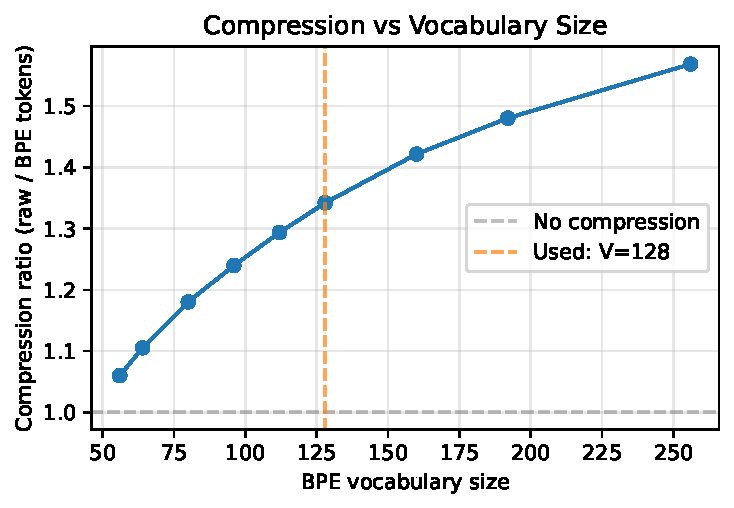
\includegraphics[width=0.55\textwidth]{compression_vs_vocab.pdf}
\caption{Compression ratio vs.\ BPE vocabulary size.  The curve is concave, with diminishing returns beyond $|\mathcal{V}| \approx 200$.  The dashed line marks the operating point $|\mathcal{V}| = 128$.}
\label{fig:compression}
\end{figure}

The modest compression --- compared to natural language BPE which routinely achieves $3$--$5\times$ --- is consistent with the high source entropy.  The HMM has an entropy rate of approximately $2.44$\,nats/token (computed via the transfer-matrix method in the Time-Reversal report).  With 48 tokens, the maximum possible entropy is $\log 48 \approx 3.87$\,nats, giving an efficiency of $2.44 / 3.87 \approx 63\%$.  A source this entropic simply does not have enough redundancy for BPE to compress aggressively.

The token frequency distribution (Figure~\ref{fig:token-freq}) shows the redistribution of probability mass.  Raw HMM tokens have a structured but moderately uniform distribution (reflecting the Dirichlet emissions within each layer).  After BPE, the distribution is spread across 128 tokens with a long tail of low-frequency merged tokens.

\begin{figure}[ht]
\centering
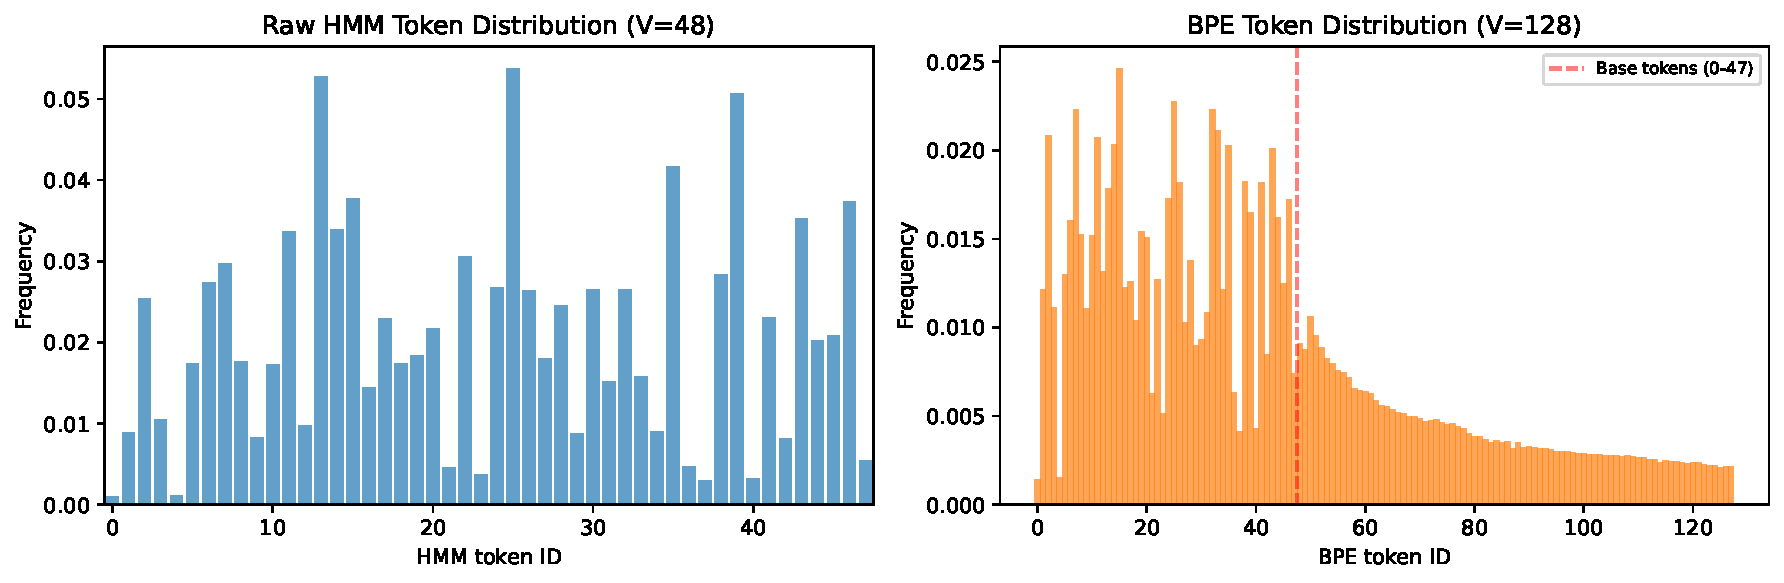
\includegraphics[width=0.95\textwidth]{token_frequencies.pdf}
\caption{Token frequency distributions.  Left: raw HMM tokens ($V = 48$), showing three-layer structure.  Right: BPE tokens ($V = 128$); base tokens (left of dashed line) lose mass to merged tokens (right), producing a long tail.}
\label{fig:token-freq}
\end{figure}

%----------------------------------------------------------------------
\section{Entropy Analysis}\label{sec:entropy}
%----------------------------------------------------------------------

BPE is a deterministic, invertible transformation: it reshapes the token sequence but cannot add or remove information.  The question is how it redistributes the prediction difficulty across tokens.

Using empirical bigram statistics on $2 \times 10^6$ tokens, we estimate bigram-approximation entropy rates for the raw and BPE-encoded sequences (Figure~\ref{fig:entropy}):

\begin{center}
\begin{tabular}{lcc}
\toprule
Representation & Entropy rate & Unit \\
\midrule
Raw HMM & 2.668 & nats/token \\
BPE & 3.508 & nats/BPE-token \\
BPE (normalised) & 2.614 & nats/raw-token \\
\bottomrule
\end{tabular}
\end{center}

The BPE entropy rate per BPE token is \emph{higher} than the raw rate (3.508 vs.\ 2.668\,nats) because each BPE token covers $\sim$1.34 raw tokens on average, packing more information per token.  When normalised to nats per raw token --- dividing by the compression ratio --- the BPE rate (2.614) is slightly \emph{below} the raw bigram rate (2.668).  This small reduction ($\sim 2\%$) reflects the bigram correlations that BPE absorbs into its merged tokens: a BPE bigram effectively conditions on a longer raw context than a raw bigram does.

\begin{figure}[ht]
\centering
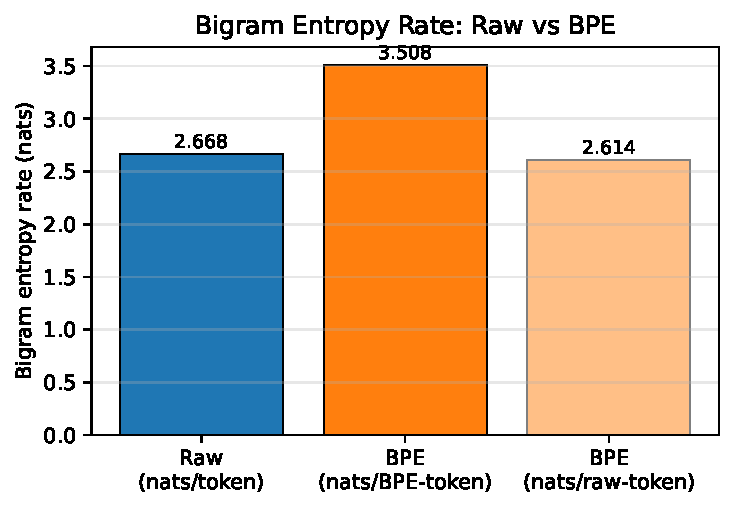
\includegraphics[width=0.5\textwidth]{entropy_rate_comparison.pdf}
\caption{Bigram entropy rates for raw and BPE representations.  The BPE rate per BPE token is higher (more information per token); normalised to raw tokens, BPE is slightly lower because it absorbs some local correlation.}
\label{fig:entropy}
\end{figure}

\paragraph{Implications for transformer training.}  The transformer trained on BPE tokens sees a context window of $T = 16$ BPE tokens, which covers $\sim$21 raw HMM tokens on average.  This extended effective context could help or hurt: it provides more raw information per window, but the prediction target is also harder (higher entropy per token).  The net effect depends on whether the additional raw context outweighs the increased per-token difficulty --- an empirical question addressed by the training experiments.

%----------------------------------------------------------------------
\section{Time-Reversal Experiment}\label{sec:reversal}
%----------------------------------------------------------------------

The BPE time-reversal experiment mirrors the raw-token reversal study from the Time-Reversal Symmetry report, but with one critical difference: reversal is performed at the \emph{BPE token level}.  Given a forward BPE sequence $(b_1, b_2, \ldots, b_T)$, the reversed sequence is $(b_T, b_{T-1}, \ldots, b_1)$.  This is \emph{not} equivalent to reversing the raw HMM tokens and then re-tokenizing, because BPE merges are learned from the forward distribution and may not decompose identically under reversal.

\subsection{Experimental Design}

\begin{itemize}
\item \textbf{Forward BPE}: raw HMM sequence $\to$ BPE encode $\to$ chunk into windows of length 17.
\item \textbf{Reversed BPE}: same BPE-encoded sequence $\to$ flip each window along the time axis.
\item Both directions use the \emph{same} tokenizer (trained on forward data) and the same compression ratio, so losses are directly comparable in nats/BPE-token.
\item Architecture and hyperparameters are identical across directions.
\item Five random seeds per direction for variance estimation.
\end{itemize}

\subsection{What Token-Level Reversal Tests}

Token-level BPE reversal confounds two effects:

\begin{enumerate}
\item \textbf{Temporal reversal of the HMM process.}  The reversed BPE sequence approximately corresponds to the time-reversed HMM, since BPE merges are local and mostly preserve temporal order within each token.

\item \textbf{Tokenizer mismatch.}  The BPE tokenizer was trained on the forward distribution.  When the model sees reversed BPE tokens, the internal n-gram structure of each token (which encodes a forward bigram) is misaligned with the reversed temporal context.  For example, a merged token representing the forward bigram $(22, 25)$ appears in the reversed sequence where the local context expects the reverse bigram $(25, 22)$.
\end{enumerate}

These two effects work in the same direction: both make reversed prediction harder.  The raw-token reversal experiment (Time-Reversal report) isolates effect~(1) alone.  Comparing the BPE reversal gap to the raw reversal gap would indicate how much additional difficulty the tokenizer mismatch contributes.

\subsection{Training Results}

Training was conducted on the cluster (6 forward seeds, 5 reversed seeds) using the architecture described in Section~\ref{sec:pipeline}.  Loss curves were downloaded from Weights \& Biases and plotted by \texttt{scripts/plot\_bpe\_dynamics.py}.

Figure~\ref{fig:bpe-dynamics} shows the validation loss over training.  The forward and reversed curves are visually indistinguishable at all training steps, with the variance bands overlapping completely.  Table~\ref{tab:bpe-results} summarises the final losses.

\begin{table}[ht]
\centering
\begin{tabular}{l c c}
\toprule
Direction & Best val loss (mean $\pm$ s.d.) & $N_{\mathrm{seeds}}$ \\
\midrule
Forward BPE & $3.321 \pm 0.003$ & 6 \\
Reversed BPE & $3.320 \pm 0.001$ & 5 \\
\midrule
$\Delta = L_{\mathrm{rev}} - L_{\mathrm{fwd}}$ & $-0.001$ & --- \\
\bottomrule
\end{tabular}
\caption{Final validation losses for BPE forward and reversed training.  The gap is consistent with zero and smaller than the cross-seed variance.}
\label{tab:bpe-results}
\end{table}

\begin{figure}[ht]
\centering
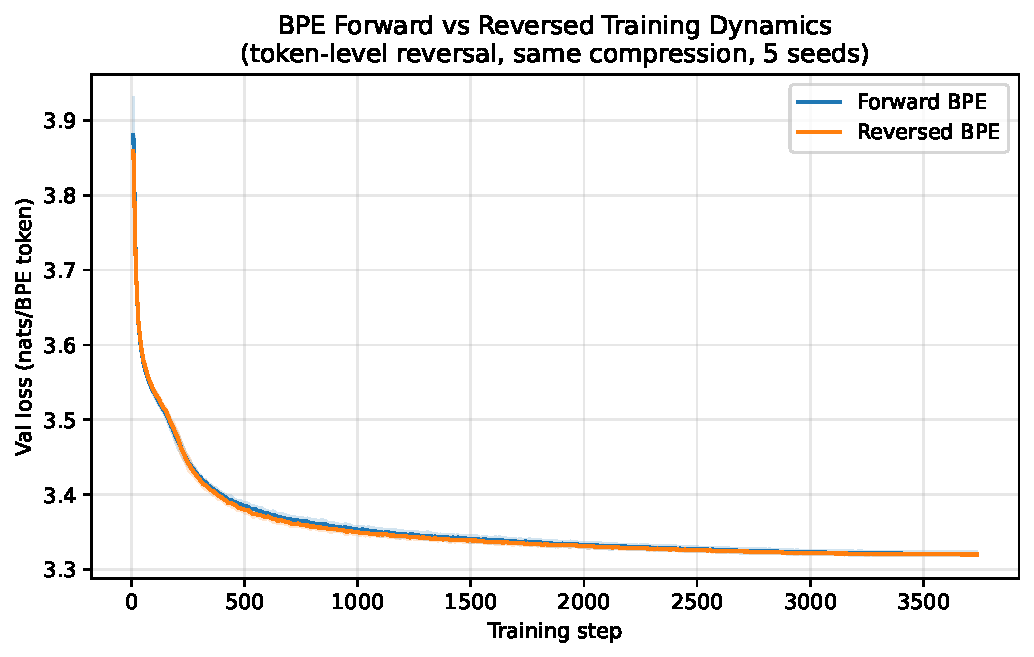
\includegraphics[width=0.75\textwidth]{bpe_training_dynamics.pdf}
\caption{BPE forward vs.\ reversed training dynamics.  Mean validation loss across seeds (solid lines) with $\pm 1$ s.d.\ bands.  The two directions are indistinguishable, consistent with the raw-token reversal result at $T = 16$.}
\label{fig:bpe-dynamics}
\end{figure}

\paragraph{Interpretation.}  The near-zero reversal gap ($\Delta \approx -0.001$\,nats, within seed variance) is consistent with the raw-token time-reversal result from the companion report.  Neither the temporal reversal of the HMM process nor the tokenizer mismatch produces a detectable effect at this context length.  This is expected: with a compression ratio of only $1.34\times$, the effective raw context ($\sim$21 tokens) is well within the regime where the Bayes-optimal gap has closed ($\Delta_{\mathrm{Bayes}}(k{=}16) = +0.0006$\,nats for raw tokens, and the BPE context covers even more raw tokens).

\paragraph{Note on mismatched runs.}  An additional batch of 6 reversed runs with 4036 steps (vs.\ 3738 for the matched runs) was found on W\&B, achieving substantially lower val loss ($\sim$3.07 vs.\ $\sim$3.32).  These runs used a different dataset chunking (likely a different \texttt{seq\_length} or data split) and are excluded from the comparison above.  The matched runs (3738 steps, identical dataset size) are the valid comparison.

%----------------------------------------------------------------------
\section{Discussion}\label{sec:discussion}
%----------------------------------------------------------------------

\subsection{BPE Discovers Emission Structure}

The most striking result of this analysis is the perfect block-diagonality of the merge table (Figure~\ref{fig:merge-layers}).  BPE, which knows nothing about hidden states or emission layers, independently recovers the partition of the observation alphabet into three emission groups.  This happens because within-layer token bigrams are far more frequent than cross-layer ones (the inter-layer transition probability is $p = 0.1$), and BPE greedily merges the most frequent pairs first.

This is reminiscent of how BPE applied to natural language discovers morphological boundaries --- here, it discovers the HMM's emission boundaries.  The analogy is instructive: in both cases, the tokenizer captures the most salient local statistical regularities of the source.

\subsection{Compression is Limited by Source Entropy}

The modest $1.34\times$ compression at $V = 128$ reflects a fundamental property of the source: the Cylinder Graph HMM is a relatively high-entropy process.  With an efficiency of $\sim$63\% relative to maximum entropy, only about a third of the token-level redundancy is available for compression.  Moreover, the redundancy that exists is primarily in within-layer bigrams, which BPE captures, but longer-range correlations (driven by the hidden state dynamics) are beyond BPE's greedy local scope.

\subsection{Open Questions}

\begin{itemize}
\item \textbf{Reversal gap magnitude.}  The BPE reversal gap ($\Delta \approx -0.001$\,nats) is comparable to the raw-token gap ($\Delta \approx +0.0002$\,nats), confirming that tokenizer mismatch does not produce a detectable additional effect at this context length.  Whether the mismatch becomes visible at shorter context or higher compression remains open.
\item \textbf{Vocabulary size sweep.}  How does the reversal gap depend on $|\mathcal{V}|$?  At $|\mathcal{V}| = 48$ (no merges), BPE reversal reduces to raw reversal; at large $|\mathcal{V}|$, the tokenizer absorbs more local structure, potentially amplifying the mismatch effect.
\item \textbf{Reverse-trained tokenizer.}  Training a BPE tokenizer on the reversed raw sequence and comparing to the forward tokenizer would isolate the tokenizer mismatch effect.
\item \textbf{Embedding geometry.}  Do BPE token embeddings exhibit the same cluster structure as raw-token embeddings?  The block-diagonal merge table suggests they should, with merged tokens interpolating between their constituent raw-token embeddings.
\end{itemize}

\end{document}
